\documentclass[12pt]{article}
\externaldocument{Comparador}
\begin{document}
\section{Malha de realimentação com retroação}

A malha de realimentação com retroação tem como objetivo recolher a informação da saída do controlador (saída do núcleo do conversor) compará-la com um sinal de referência e corrigir a saída caso esta se esteja a desviar dos parâmetros pretendidos.
A malha de realimentação é composta por :
\vspace*{5mm}

- Divisor de tensão

- Comparador com latch                                                                                                   

\subsection{Divisor de tensão resistivo}

O divisor de tensão resistivo está colocado à saída do núcleo do conversor, este tem como função diminuir a tensão do mesmo, neste caso, para que seja possível obter uma tensão de 0.5 [V] á entrada do comparador.
Na figura \ref{fig:divisor} está representado o divisor  de tensão resistivo, sendo necessário calcular os valores de $R_A$ e $R_B$. 
\vspace*{5mm}


\begin{figure}[htbp]
	\centering
	\begin{minipage}{.5\textwidth}
		\centering
		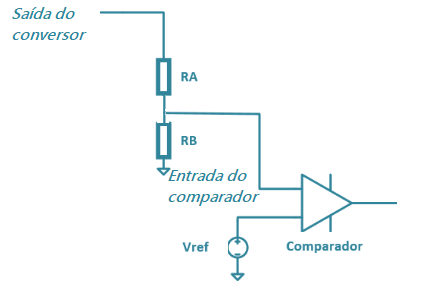
\includegraphics[height=4.5cm]{divisor}
	\caption{Divisor resistivo}
	\label{fig:divisor}
	\end{minipage}%
	\begin{minipage}{.5\textwidth}
		\centering
		{\footnotesize \begin{equation}
			\label{eq:divisorres}
			 V{o_{convensor}} =(\frac{R_B}{R_B + R_A})\times V{i_{comparador}}
		\end{equation}} 
	\end{minipage}
\end{figure}

Sabendo que :
\begin{itemize}
\item \begin{center} $V{o_{convensor}} = 0.6$ [V] \end{center}
\item \begin{center} $V{i_{comparador}} = 0.5$ [V] \end{center}
\end{itemize}
\vspace*{5mm}

Assumindo $R_B$ = 500 $[\Omega]$, resolvendo a equação \ref{eq:divisorres} em ordem a $R_A$ obtém-se: 
\begin{equation}
 R_A = \frac{R_B - (R_B \times \frac{0.6}{0.5})}{\frac{0.6}{0.5}} = 100 [\Omega]
\end{equation} 

\subsection{Comparador com latch}



Como foi referido na secção \ref{sec:comparador} o comparador irá trabalhar em duas fases distintas consoante o valor de CLK (fase Reset e fase de comparação). Na fase de comparação, o comparador irá comparar a tensão de referência $ 0.5 $ [V] com o sinal à saída do divisor resistivo. Quando a tensão a saída do divisor resistivo está abaixo da tensão de referência, $Vo_{p}$ encontra-se a VDD, enquanto que $Vo_{n}$ está a zero, a partir do momento em que são iguais há uma inversão de sinal. É de salientar que sempre que as duas tensões são iguais há uma mudança de sinal nas duas saídas do comparador e estas encontram-se em oposição uma em relação à outra. 

Na figura \ref{fig:saida_c_latch} encontra-se representada a tensão de referência a azul, o sinal à saída do divisor resistivo a rosa, $Vo_{n}$ a a laranja e $Vo_{p}$ a  a roxo. É possível verificar o comportamento do comparador descrito em cima quando as duas tensões são iguais.  

\begin{figure}[htbp]
	\centering
	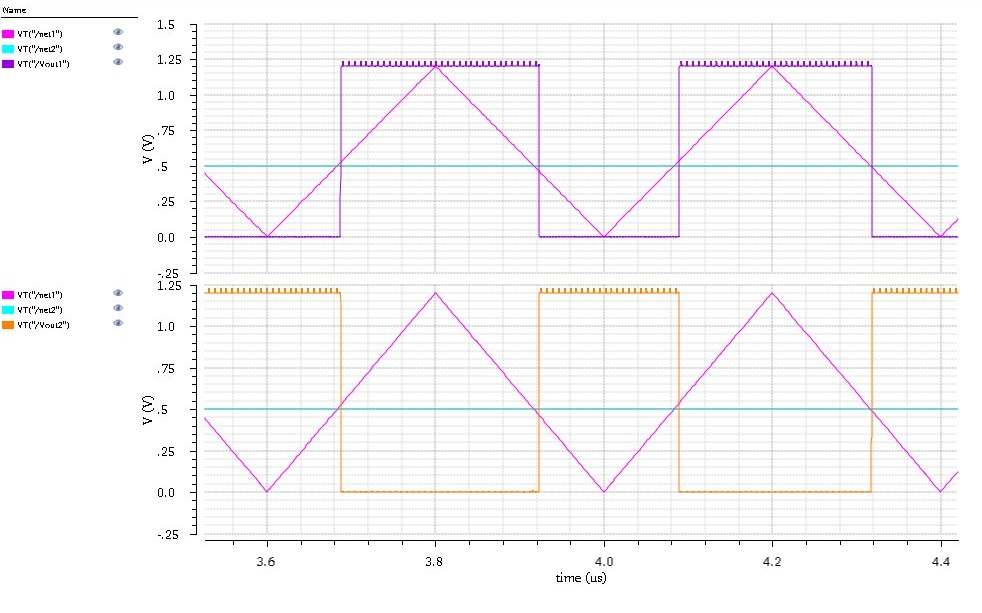
\includegraphics[width=0.7\linewidth, height=7cm]{ComparadorLatch}
	\caption{Ondas à entrada e à saída do comparador }
	\label{fig:saida_c_latch}
\end{figure}
  


\end{document}